\documentclass{article}
\usepackage[utf8]{inputenc}
\usepackage[hidelinks]{hyperref}
\usepackage[spanish]{babel}
\usepackage[left=2cm,right=2cm,top=2cm,bottom=2cm]{geometry}
\usepackage{graphicx}
\usepackage{pdflscape}
\usepackage{listings}

\lstset {
    frame = single,
    breaklines = true
}

\begin{document}
\begin{titlepage}
\title{\textbf{
    {\Huge Práctica 3: Informes y consultas sobre un Data Mart}\\
    {\Large Almacenes y Minería de Datos}
}}
\author{
    Pedro Allué Tamargo (758267)
    \and
    Cristina Oriol García (755922)
    \and
    Alejandro Paricio García (761783)
}
\date{\today}
\clearpage\maketitle
\thispagestyle{empty}
\end{titlepage}

% Index
\tableofcontents

\newpage
\section{Introducción}

En esta práctica se va a realizar la explotación del \textit{Data Mart} creado en prácticas anteriores. La explotación es una parte importante del ciclo de vida del mismo, ya que el \textit{Data Mart}, en el que se ha invertido una gran cantidad de tiempo, normalmente traducido en esfuerzo económico, va a ser un pilar fundamental en la toma de decisiones para una o varias empresas y organizaciones. En este caso, y como se comentó en prácticas anteriores, para supuestos dirigentes o personas con gran importancia de empresas relacionadas con el mundo de los vuelos comerciales en Estados Unidos. La explotación del \textit{Data Mart} tiene que dar una visión a nivel global del estado del proceso de negocio, y, durante los siguientes apartados, se extraerá información para ejemplificarlo. Se aprovecharán los nuevos conocimientos acerca de creación de consultas a almacenes de datos con éste propósito.\\


\section{Consultas básicas}

\subsection{Consulta 1}
Se desea obtener el retraso medio de los vuelos que salen de cada aeropuerto en función de la ciudad destino, junto con el retraso medio total por aeropuerto origen (con independencia del destino). Se han planteado dos alternativas para resolver este problema, una de ellas con los operadores SQL vistos en asignaturas previas, y otro con los nuevos y potentes operadores. Fácilmente podrían extraerse otras alternativas utilizando GROUPING SET en lugar de ROLL UP. Al no considerare único el nombre del aeropuerto, se requiere llevar a cabo el GROUP BY por el identificador del mismo y luego encontrar sus respectivos nombres, si no se requerie el nombre se puede mantener únicamente la primera tabla del FROM más externo.

\textbf{Alternativa 1}
\begin{lstlisting}
SELECT *
FROM (	SELECT v.IDAEROPUERTOORIGEN, a.CIUDAD, AVG(V.TIEMPODERETRASOLLEGADA) AS RetrasoMedioAeroOrigenCiudadDestino
		FROM VUELOS v JOIN AEROPUERTO a ON v.IDAEROPUERTODESTINO = a.IDAEROPUERTO 
		GROUP BY v.IDAEROPUERTOORIGEN, a.CIUDAD 
		UNION
		SELECT v2.IDAEROPUERTOORIGEN, NULL,  AVG(v2.TIEMPODERETRASOLLEGADA) AS RetrasoAeroOrigenMedioTotal
		FROM VUELOS v2 
		GROUP BY v2.IDAEROPUERTOORIGEN ) t, AEROPUERTO a2
WHERE a2.IDAEROPUERTO = t.IDAEROPUERTOORIGEN;
\end{lstlisting}

\textbf{Alternativa 2}
\begin{lstlisting}
SELECT *
FROM (	SELECT vuelo.IDAEROPUERTOORIGEN, aeropuerto.CIUDAD AS ciudadDestino, AVG(vuelo.TIEMPODERETRASOLLEGADA) AS RetrasoMedioAeropuertoOrigenCiudadDestino
		FROM Vuelos vuelo JOIN AEROPUERTO aeropuerto ON vuelo.IDAEROPUERTODESTINO = aeropuerto.IDAEROPUERTO 
		GROUP BY ROLLUP(vuelo.IDAEROPUERTOORIGEN, aeropuerto.CIUDAD)
		HAVING GROUPING(vuelo.IDAEROPUERTOORIGEN) != 1 OR GROUPING(aeropuerto.CIUDAD) != 1 ) t, AEROPUERTO a2
WHERE a2.IDAEROPUERTO = t.IDAEROPUERTOORIGEN;
\end{lstlisting}

\newpage
\subsection{Consulta 2}

Obtener el retraso medio de los vuelos que salen de cada aeropuerto en función de la ciudad destino, junto con el retraso medio total por aeropuerto origen (con independencia del destino) y el retraso medio total por destino (con independencia del aeropuerto origen).  Al igual que en la consulta anterior, y de aquí en adelante, al no considerare único el nombre del aeropuerto, se requiere llevar a cabo el GROUP BY por el identificador del mismo y luego encontrar sus respectivos nombres, si no se requerie el nombre se puede mantener únicamente la primera tabla del FROM más externo\\

El número de resultados obtenidos son los 5891 de la consulta anterior + el nuevo conjunto, que es, en este caso, el resultado de agrupar por ciudades destino (345).\\

\textbf{Alternativa 1}
\begin{lstlisting}
SELECT *
FROM (	SELECT vuelo.IDAEROPUERTOORIGEN, aeropuerto.CIUDAD AS ciudadDestino, AVG(vuelo.TIEMPODERETRASOLLEGADA) AS RetrasoMedioAeropuertoOrigenCiudadDestino
		FROM Vuelos vuelo JOIN AEROPUERTO aeropuerto ON vuelo.IDAEROPUERTODESTINO = aeropuerto.IDAEROPUERTO 
		GROUP BY CUBE(vuelo.IDAEROPUERTOORIGEN, aeropuerto.CIUDAD)
		HAVING GROUPING(vuelo.IDAEROPUERTOORIGEN) != 1 OR GROUPING(aeropuerto.CIUDAD) != 1) t, AEROPUERTO a2
WHERE a2.IDAEROPUERTO = t.IDAEROPUERTOORIGEN;
\end{lstlisting}


\textbf{Alternativa 2}
\begin{lstlisting}
SELECT *
FROM (	SELECT v.IDAEROPUERTOORIGEN, a.CIUDAD, AVG(V.TIEMPODERETRASOLLEGADA) AS RetrasoMedioAeroOrigenCiudadDestino
		FROM VUELOS v JOIN AEROPUERTO a ON v.IDAEROPUERTODESTINO = a.IDAEROPUERTO 
		GROUP BY v.IDAEROPUERTOORIGEN, a.CIUDAD
		UNION
		SELECT v2.IDAEROPUERTOORIGEN, NULL, AVG(v2.TIEMPODERETRASOLLEGADA) AS RetrasoAeroOrigenMedioTotal
		FROM VUELOS v2 
		GROUP BY v2.IDAEROPUERTOORIGEN 
		UNION
		SELECT NULL, a2.CIUDAD, AVG(v3.TIEMPODERETRASOLLEGADA) AS RetrasoAeroDestinoMedioTotal
		FROM VUELOS v3 JOIN AEROPUERTO a2 ON v3.IDAEROPUERTODESTINO = a2.IDAEROPUERTO 
		GROUP BY a2.CIUDAD ) t, AEROPUERTO a2
WHERE a2.IDAEROPUERTO = t.IDAEROPUERTOORIGEN;
\end{lstlisting}


\newpage
\section{Consultas propias}

\subsection{Consulta 1}
Obtener el tiempo real de vuelo medio de los vuelos en función de su estado de origen y la aerolínea a cargo del mismo, así como  el tiempo real de vuelo medio de los vuelos  en función de su estado de destino y la aerolínea a cargo del mismo.\\

No hay problemas con los \textit{NULLS} en la clásulua where, porque todos los grouping set abarcan a la aerolínea, por lo que el where de después no se topa con valores de éste tipo en ese campo. Se aprovecha que el \textit{IDAEROLINEA} aparece en ambos grupos. En esta ocasión, para resolver la consulta se ha acudido a los \textit{GROUPING SETS}.

\begin{lstlisting}
SELECT *
FROM ( SELECT v.IDAEROLINEA AS idAerolinea, aero.ESTADO AS estadoDestino, aero2.ESTADO AS estadoOrigen, 
				AVG(v.TIEMPOREALVUELO) AS mediaTiempoRealVuelo, GROUPING_ID(aero.ESTADO, aero2.ESTADO) 
	   FROM VUELOS v JOIN AEROPUERTO aero ON aero.IDAEROPUERTO = v.IDAEROPUERTODESTINO JOIN AEROPUERTO aero2 
	   			ON aero2.IDAEROPUERTO = v.IDAEROPUERTOORIGEN 
	   GROUP BY GROUPING SETS ((v.IDAEROLINEA, aero.ESTADO), (v.IDAEROLINEA, aero2.ESTADO)) ) vuelos, Aerolinea aerolinea 
WHERE vuelos.IDAEROLINEA = aerolinea.IDAEROLINEA;
\end{lstlisting}


\subsection{Consulta 2}
Se desea conocer la aerolínea que ha gestionado más vuelos que en función de su estado ciudad y aeropuerto de origen, en función de su estado y ciudad y de únicamente su estado, así como el número de los vuelos que gestiona en cada caso.\\

Para solventar esta consulta se ha empleado un \textit{ROLL UP} parcial, que nos permite obtener los grupos (nombre aerolinea, estado, ciudad, nombre aeropuerto), (nombre aerolinea, estado, ciudad) y (nombre aerolinea, estado). Pese al no considerarse único el nombre de la aerolínea, nuestro conocimiento de los datos nos permite saber que en la primera y única carga a realizar, las aerolíneas cuyo nombre coincidía tienen su nombre modificado, añadiendo a la segunda de las mismas el sufijo \textit{(1)}, por tanto, no se repiten. De ésta forma podemos consultar directamente agrupando por el nombre de la aerolínea, simplificando la consulta. Necesario comentar que hay que tener un amplio conocimiento de los datos utilizados para poder llevar a cabo este tipo de simplificaciones sin cometer errores.

\begin{lstlisting}
SELECT origen.NOMBREAEROLINEA, origen.ESTADO, origen.CIUDAD, origen.NOMBREAEROPUERTO, COUNT(*)
FROM (SELECT * FROM (VUELOS v  JOIN AEROPUERTO a ON a.IDAEROPUERTO = v.IDAEROPUERTOORIGEN) 
							   JOIN AEROLINEA a2 ON a2.IDAEROLINEA = v.IDAEROLINEA) origen
GROUP BY origen.NOMBREAEROLINEA, origen.ESTADO, ROLLUP(origen.CIUDAD, origen.NOMBREAEROPUERTO);

\end{lstlisting}


\newpage
\subsection{Consulta 3}

Obtener el número de vuelos que aterrizan en cada estado y en función de la operadora por la que están gestionados. Obtener además el número de vuelos totales que aterrizan en cada estado y el número de vuelos que gestiona cada operadora. Únicamente se desea mostrar esa información, no mostrándose información adicional alguna.\\

En esta tercera consulta se ha recurrido al operador \textit{CUBE}, que extraerá los grupos (o.IDOPERADORA , a.ESTADO), (o.IDOPERADORA), (a.ESTADO) y (). No obstante, el último no se desea mostrar, por lo que se ha recurrido a GROUPING para asegurar que al menos 1 de los dos atributos no es nulo.\\

\textbf{Alternativa 1}
\begin{lstlisting}
SELECT *
FROM ( SELECT o.IDOPERADORA , a.ESTADO, COUNT(*) AS numVuelos
       FROM (VUELOS v JOIN AEROPUERTO a ON a.IDAEROPUERTO = v.IDAEROPUERTODESTINO) JOIN OPERADORA o ON o.IDOPERADORA = v.IDOPERADORA 
       GROUP BY CUBE(o.IDOPERADORA , a.ESTADO)
       HAVING GROUPING(o.IDOPERADORA) != 1 OR GROUPING(a.ESTADO) != 1 ) tienda
       LEFT OUTER JOIN OPERADORA o2 ON o2.IDOPERADORA = tienda.IDOPERADORA;
\end{lstlisting}

\textbf{Alternativa 2}
\begin{lstlisting}
SELECT *
FROM  ( SELECT v.IDOPERADORA, a.ESTADO, COUNT(*) AS numVuelos
        FROM VUELOS v JOIN AEROPUERTO a ON a.IDAEROPUERTO = v.IDAEROPUERTODESTINO 
        GROUP BY GROUPING SETS((v.IDOPERADORA, a.ESTADO), (v.IDOPERADORA), (a.ESTADO)) ) tienda
        LEFT OUTER JOIN OPERADORA o2 ON o2.IDOPERADORA = tienda.IDOPERADORA;
\end{lstlisting}

Una tercera alternativa sería empleando múltiples \textit{UNION}, como en la primera y segunda consultas obligatoria.


\subsection{Consulta 4}
Obtener la media de tiempo real de vuelo de los vuelos que parten de cada uno de los aeropuertos en función de su estado. Además, también se debe incluir la media de los vuelos de todos los aeropuertos de cada estado y del total de vuelos del país. Quiero también que, para cada subgrupo, exista un ranking de los aeropuertos en función de la mencionada media.\\

La primera parte de la consulta consiste únicamente en un \textit{ROLL UP} simple. La segunda parte del mismo, sin embargo, es complicada de llevar a cabo con los operadores empleados hasta ahora. Por ello, se utilizará el operador \textit{RANK} ~\cite{rank:1} ~\cite{rank:2}, que permite calcular un ranking para cada fila dentro de una partición del conjunto de resultados. Aquellos miembros de un mismo grupo con la misma media tendrán el mismo valor en el ranking.

\begin{lstlisting}
SELECT origen.ESTADO, origen.NOMBREAEROPUERTO, AVG(origen.TIEMPOREALVUELO), RANK() OVER ( 
			PARTITION BY origen.ESTADO ORDER BY AVG(origen.TIEMPOREALVUELO) DESC) rankingTiempoVuelo
FROM (SELECT * FROM (VUELOS v  JOIN AEROPUERTO a ON a.IDAEROPUERTO = v.IDAEROPUERTOORIGEN)) origen
GROUP BY ROLLUP(origen.ESTADO, origen.NOMBREAEROPUERTO);
\end{lstlisting}


\newpage
\subsection{Consulta 5}
Obtener el número de aviones con retraso a la salida en función de su estado, ciudad, aeropuerto (de salida, obviamente) y su aerolínea. También se desea conocer el número de aviones con retraso a la salida en función de su estado, ciudad y aeropuerto, de su estado y ciudad y únicamente de su estado. Se desea también poder identificar fácilmente qué campos no se están teniendo en cuenta para la agrupación en cada fila y que no se muestre más información de la estrictamente pedida.\\

De nuevo se plantean dos alternativas, que emplean \textit{ROLL UP} parcial. Una de ellas muestra identificadores de la aerolínea y aeropuerto, mientras que en la otra se han incluido \textit{LEFT OUTER JOINs} para añadir los nombres en cadena de texto tratando los NULLS correctamente.\\


\textbf{Alternativa 1}
\begin{lstlisting}
SELECT a.ESTADO, a.CIUDAD, v.IDAEROPUERTOORIGEN, v.IDAEROLINEA, GROUPING_ID(a.CIUDAD, v.IDAEROPUERTOORIGEN, v.IDAEROLINEA), COUNT(*) AS cuenta
FROM VUELOS v JOIN AEROPUERTO a ON a.IDAEROPUERTO = v.IDAEROPUERTOORIGEN 
WHERE TIEMPODERETRASOSALIDA > 0
GROUP BY a.ESTADO, ROLLUP(a.CIUDAD, v.IDAEROPUERTOORIGEN, v.IDAEROLINEA);
\end{lstlisting}

\textbf{Alternativa 2}
\begin{lstlisting}
SELECT tabla.ESTADO, tabla.CIUDAD, tabla.NOMBREAEROPUERTO, tabla.IDAEROPUERTOORIGEN, tabla.IDAEROLINEA, tabla.groupingId, tabla.cuenta, a3.CODIGOAEROLINEA, a3.NOMBREAEROLINEA 
FROM ( SELECT tienda.ESTADO, tienda.CIUDAD, a2.NOMBREAEROPUERTO, tienda.IDAEROPUERTOORIGEN, tienda.IDAEROLINEA, tienda.groupingId, tienda.cuenta
		FROM(   SELECT a.ESTADO, a.CIUDAD, v.IDAEROPUERTOORIGEN, v.IDAEROLINEA, GROUPING_ID(a.CIUDAD, v.IDAEROPUERTOORIGEN, v.IDAEROLINEA) AS groupingId, COUNT(*) AS cuenta
				FROM VUELOS v JOIN AEROPUERTO a ON a.IDAEROPUERTO = v.IDAEROPUERTOORIGEN 
				WHERE TIEMPODERETRASOSALIDA > 0
				GROUP BY a.ESTADO, ROLLUP(a.CIUDAD, v.IDAEROPUERTOORIGEN, v.IDAEROLINEA) ) tienda LEFT OUTER JOIN AEROPUERTO a2 ON a2.IDAEROPUERTO = tienda.IDAEROPUERTOORIGEN ) tabla
		LEFT OUTER JOIN AEROLINEA a3 ON a3.IDAEROLINEA = tabla.IDAEROLINEA
\end{lstlisting}


\section{Sentencia \texttt{CREATE DIMENSION}}

La sentencia \texttt{CREATE DIMENSION} de \textit{Oracle} se utiliza para la creación de dimensiones en este sistema gestor de bases de datos. Esta es una de las sentencias utilizadas en \textit{Oracle} para dar una capa de abstracción adicional sobre el \textit{SQL} y obtener una visión similar al esquema en estrella desarrollado. Esta sentencia se basa en la creación de relaciones \textit{``padre-hijo''} entre columnas.\\
En la documentación de \textit{Oracle\footnote{\url{https://docs.oracle.com/cd/B19306_01/server.102/b14200/statements_5006.htm}}} se puede observar la semántica de la operación y distintos ejemplos de utilización.\\


\newpage
\section{Creación de informes y cuadros de mando}

Para la generación de informes y cuadros de mando se va a utilizar la herramienta \textit{PowerBI\footnote{\url{https://powerbi.microsoft.com/es-es/}}} de \textit{Microsoft}. \textit{PowerBI} es una herramienta de \textit{Business Intelligence} utilizada en la industria y permite la creación de visualizaciones a partir de datos y un modelo estructurado de los mismos. Se ha elegido esta herramienta debido a su previa utilización de uno de los integrantes del equipo.\\
Esta herramienta permite obtener los datos de diversas fuentes de datos tales como bases de datos, ficheros de texto, hojas de cálculo de \textit{Excel}... En este caso se va a utilizar la base de datos \textit{Oracle} situada en \textit{danae04}, en esta base de datos se han introducido todos los datos del \textit{Data Mart} diseñado y poblado en prácticas anteriores.\\


\subsection{Instalación y preparación de \textit{PowerBI}}

Para instalar \textit{PowerBI} y evitar problemas con los drivers de \textit{Oracle} se va a instalar desde la su centro de descargas\footnote{\url{https://www.microsoft.com/en-us/download/details.aspx?id=58494}}. Una vez descargada e instalada la herramienta se va a proceder a instalar el cliente de \textit{Oracle} para \textit{Windows\footnote{Para la versión de 64 bits el enlace sería: \url{https://www.oracle.com/database/technologies/odac-downloads.html}}}. Hay que descargar el fichero \textit{ODACXXXXXXXXXXx64.zip}~\cite{ms:1}. Para instalar el cliente de \textit{Oracle} hay que ejecutar el fichero ejecutable \texttt{install.bat} \textit{all path myhome} \texttt{true true}. El instalador no añade a la variable de entorno \textit{PATH} las rutas \textit{path} y \textit{path/bin}. Para configurar la conexión con la base de datos se va a proveer un alias a la base de datos \textit{Oracle}. Para ello se va a crear un fichero \textit{tnsnames.ora} en el directorio \textit{path}\texttt{/network/admin/}. El contenido del fichero será el siguiente:

\begin{lstlisting}
danae04 =
  (DESCRIPTION =
    (ADDRESS = (PROTOCOL = TCP)(HOST = danae04.unizar.es)(PORT = 1521))
    (CONNECT_DATA =
      (SERVER = DEDICATED)
      (SERVICE_NAME = barret)
    )
  )
\end{lstlisting}

Una vez configurada la herramienta se va a proceder a la configuración e importación de datos de la base de datos. Para importar los datos se seleccionará la opción: \textit{``Obtener datos``} y en el menú se seleccionará \textit{Bases de Datos $\rightarrow$ Oracle Database}. En el cuadro de texto de la Figura \ref{fig:cuadroConexion} se introducirá el alias asignado anteriormente en el fichero \textit{tnsnames.ora} (\textit{danae04}). Tras esto, la herramienta \textit{PowerBI} pedirá las credenciales de autenticación del usuario en \textit{Windows}. En la Figura \ref{fig:cuadroConexionCredenciales} se puede observar que aparece la opción de \textit{Base de Datos} para autenticarse directamente en la base de datos. Se utilizará esta última opción.\\
Tras la autenticación se abrirá una ventana para seleccionar las tablas que se desean importar. Este paso puede tardar mucho tiempo. Durante la realización de la prácticas se tardó cerca de 15 minutos en conseguir que la herramienta mostrara las tablas para el esquema \textit{A758267}.\\
La importación de los datos también costó mucho tiempo. La herramienta intentaba cargar los datos de las tablas seleccionadas y a los 10 minutos se cancelaba la operación mostrando un error de \textit{Oracle} (\textit{The gateway operation has been cancelled explicitly by the user or from a timeout}). Al reintentarlo se consiguieron importar correctamente todos los datos.\\


\newpage
\subsection{Modelo de datos}

Como se ha comentado anteriormente la herramienta \textit{PowerBI} genera un modelo estructurado de datos (como una base de datos). Este modelo puede ser modificado por el usuario para incluir relaciones que la herramienta no ha detectado. En este caso no ha sido necesario añadir ninguna relación adicional. El modelo de datos de \textit{PowerBI} se puede observar en la Figura \ref{fig:modeloDatos}.\\


\subsection{Generación de cuadros de mando}

Utilizando la herramienta anterior se va a proceder a crear cuadros de mando \textit{dashboards} útiles para los usuarios del almacén de datos y que permitan obtener información clara acerca del estado del proceso de negocio que se está manejando. Se han desarrollado dos \textit{dashboards} para este proceso, cada uno se centrará en mostrar información de los retrasos y tiempos de vuelo agrupados por distintos elementos.\\

\subsubsection{Cuadro de mando del estado de las aerolíneas}

Se ha confeccionado un cuadro de mando relativo a la información de los tiempos de retraso y de vuelo relacionados con las aerolíneas que operan en estados unidos. En la Figura \ref{fig:dashboardAerolineas} se pueden observar 3 visualizaciones. Estas visualizaciones son interactivas, es decir, si se interactúa con alguna de las situadas en la mitad superior se pueden obtener los datos relacionados con esta aerolínea (se resaltan los datos en las otras gráficas).\\

\begin{figure}[h!]
    \centering
    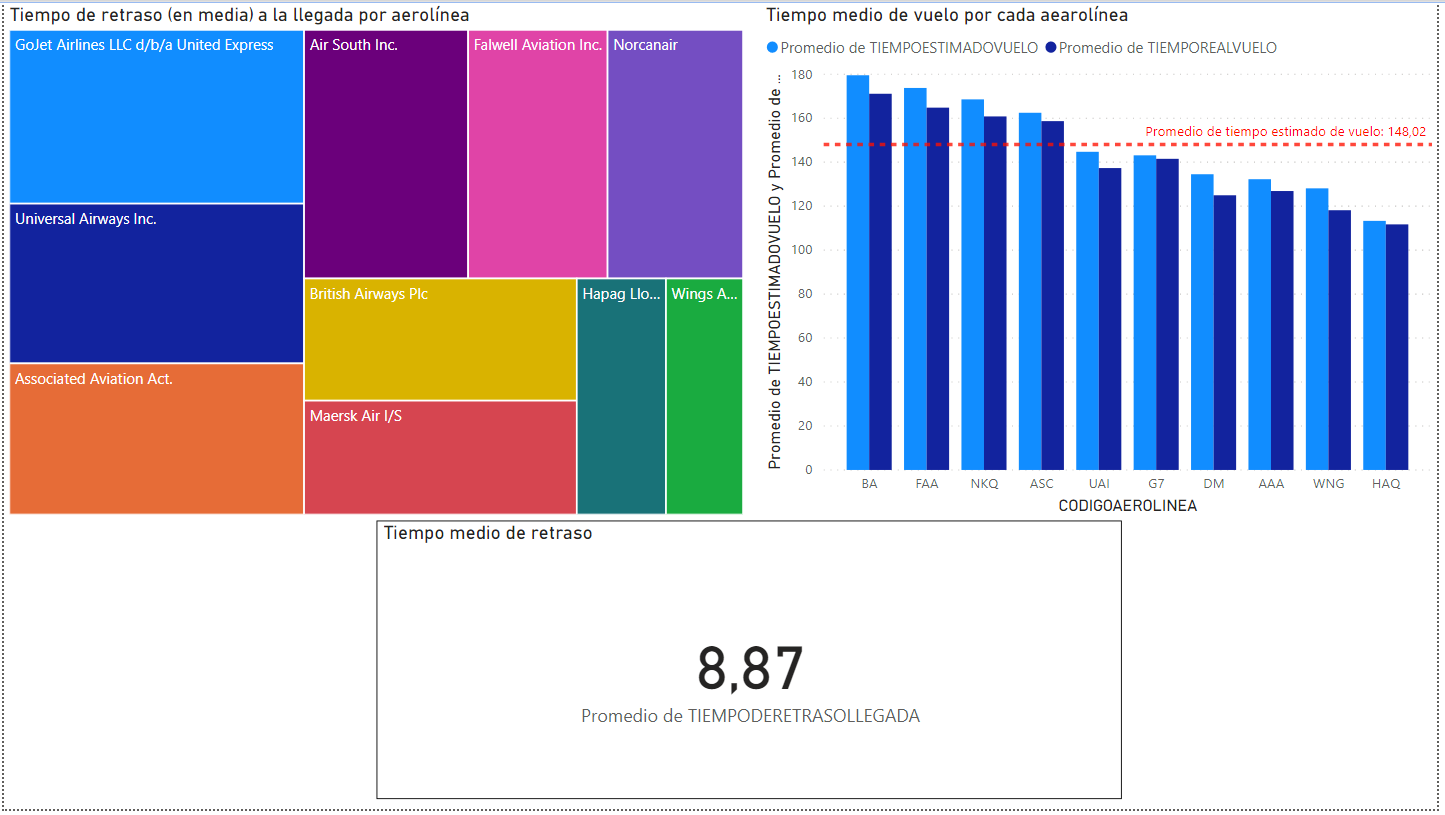
\includegraphics[scale=0.5]{images/cuadroPedro.png}
    \caption{Captura de pantalla del cuadro de mando de comparación de aerolíneas}
    \label{fig:dashboardAerolineas}
\end{figure}

Este cuadro de mando está disponible públicamente en la plataforma de \textit{PowerBI} mediante el siguiente \href{https://app.powerbi.com/view?r=eyJrIjoiODUwZTA1MmMtMWIwOS00MTVlLWFlYzUtZmI5YzgwMzFhNDY5IiwidCI6IjNmMjI3ZGJhLWYzZjQtNDU0NC1iMzE0LWM2ZWZkMzBlMGQwMCIsImMiOjh9}{\textit{enlace}}. También se puede encontrar en el fichero \texttt{amdp3.pbix}.\\


\newpage
\subsubsection{Cuadro de mando del estado de los vuelos en cada ciudad}
Se ha creado un cuadro de mando en el que se pueden observar los tiempos de retraso medio de los vuelos relacionados con las ciudades a las que pertenecen los distintos aeropuertos de origen de estos. Como visualizamos en la figura \ref{fig:dashboardCiudades} estos datos son presentados mediante un mapa en el que aparecen marcadas las ciudades de las cuales hay disponible información respecto a los vuelos y una gráfica en la que aparecen las ciudades con un mayor retraso tanto en su salida como en la llegada al origen. Como añadido podemos ver dos visualizaciones más, una nos da información sobre el porcentaje total de los vuelos que han sufrido retraso y los que no, la otra nos ofrece el retraso en minutos promedio que sufren los vuelos. Son visualizaciones interactivas lo que significa que si en el mapa interactúa con alguna de las ciudades el resto de gráficas cambiará para ofrecernos la información exclusivamente relativa a esta ciudad ,aunque la visualización del porcentaje no proporciona información funcional, las otras dos si nos ofrecen los datos ya explicados en la gráfica y la media de retraso en sus vuelos.


\begin{figure}[h!]
    \centering
    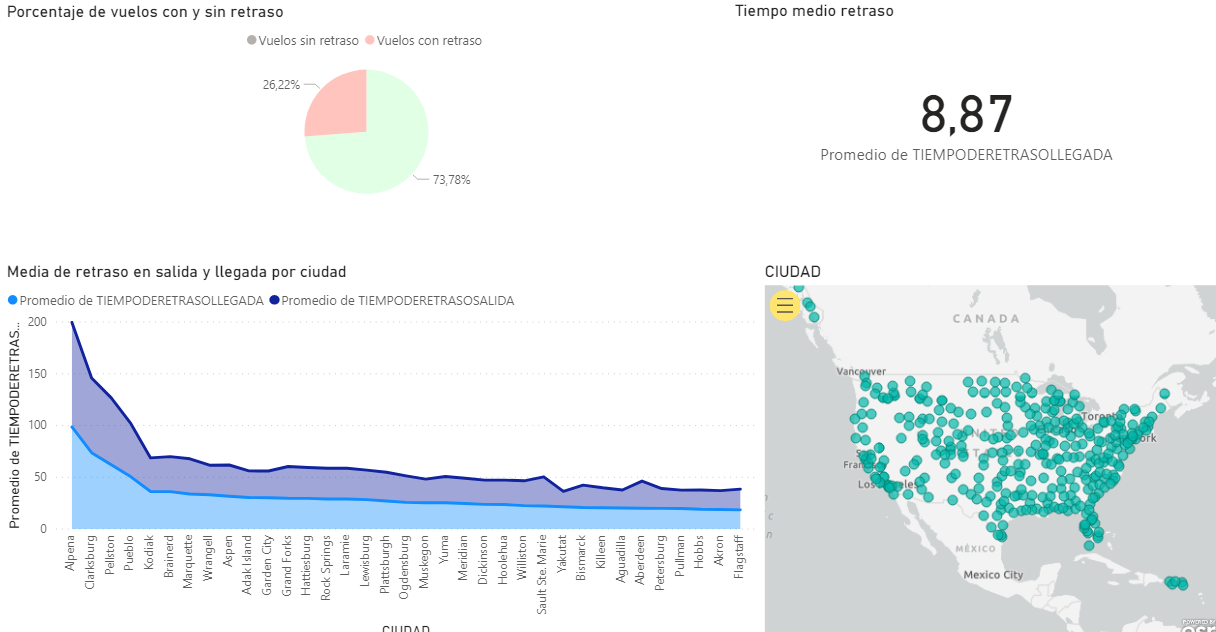
\includegraphics[scale=0.5]{images/cuadrocris.png}
    \caption{Captura de pantalla del cuadro de mando de comparación de ciudades}
    \label{fig:dashboardCiudades}
\end{figure}

Este cuadro de mando está disponible públicamente en la plataforma de \textit{PowerBI} mediante el siguiente \href{https://app.powerbi.com/view?r=eyJrIjoiYzJkMWI2MmQtZWI4OC00NGM5LTg4NDEtZWVhZTVmM2I2NmMzIiwidCI6IjNmMjI3ZGJhLWYzZjQtNDU0NC1iMzE0LWM2ZWZkMzBlMGQwMCIsImMiOjh9}{\textit{enlace}}, aunque en este el mapa no se visualiza correctamente mientras en la aplicación de PowerBi sí funciona correctamente. También se puede encontrar en el fichero \texttt{amdp3-2.pbix}.\\


\newpage
\section{Conclusiones y dificultades encontradas}

Durante la realización de las consultas SQL, caben destacar dos aspectos principales, que han sido considerados como los más relevantes. El primero de ellos es el gran potencial de los operadores de análisis como \textit{CUBE}, \textit{ROLL UP} y \textit{GROUPING SETS}. Gracias a ello es posible llevar a cabo consultas inicialmente complejas mediante un conjunto de cláusulas SQL mucho más sencillo. Se ilustra este comportamiento en las consultas en las que se han obtenido múltiples alternativas, al menos una empleando estos operadores, y al menos otra sin utilizarlos, como, por ejemplo, en la segunda consulta obligatoria. El otro elemento destacable es la dificultad añadida con la necesidad del tratamiento de los \textit{NULL} en algunas consultas. Al utilizar los operadores anteriores, aparecen valores \textit{NULL}, que al hacer \textit{JOIN} con otras tablas, pueden dar como resultado algo incorrecto. Por ello, son importantes los operadores de tipo \textit{OUTER JOIN}, como el \textit{LEFT OUTER JOIN}. Además, cobra gran importancia la presencia o ausencia de valores nulos en el almacén de datos. En nuestro caso hemos conseguido que no aparezcan, evadiéndose así esa posibilidad, pero, de otra manera, habría que tenerlos enc uenta de forma explícita en algunas consultas. Llevar a cabo todas las consultas anteriores ha permitido que ambos elementos se pongan de manifiesto, destacándose especialmente el potencial del primero, así como las opciones al utilizar dichos operadores, como podrían ser los \textit{ROLL UP} o \textit{CUBE} parciales.\\
En la parte de la creación de informes se han experimentado problemas con la carga de datos desde la base de datos de \textit{Oracle}, también ha habido diversos problemas durante la instalación del cliente de Oracle por errores durante el proceso de instalación. Este problema realentizó mucho el inicio de la creación de cuadros de mando hasta tal punto que se propuso la utilización de \textit{Tableau\footnote{\url{https://www.tableau.com/es-es}}}. \textit{PowerBI} es una herramienta muy potente para la creación de visualizaciones y muy intuitiva de cara al usuario por lo que su aprendizaje no ha sido un impedimento de cara a su uso en esta práctica.\\

\subsection{Control de esfuerzos}
\begin{itemize}
    \item Pedro Allué Tamargo: Creación de consultas básicas, instalación de PowerBI, integración de Oracle con PowerBI, creación de cuadros de mando, redacción de la memoria:
        \begin{itemize}
            \item Tiempo invertido: 11 horas
        \end{itemize}
    \item Cristina Oriol García: Creación de consultas básicas, creación de cuadros de mando, redacción de la memoria. 
        \begin{itemize}
            \item Tiempo invertido: 9 horas
        \end{itemize}
    \item Alejandro Paricio García:
        \begin{itemize}
            \item Tiempo invertido: 11 horas
        \end{itemize}
\end{itemize}

% Anexo de figuras
\newpage
\section{Anexo 1: Figuras}

\subsection{Cuadro de conexión de \textit{PowerBI} con \textit{Oracle}}

\begin{figure}[h!]
    \centering
    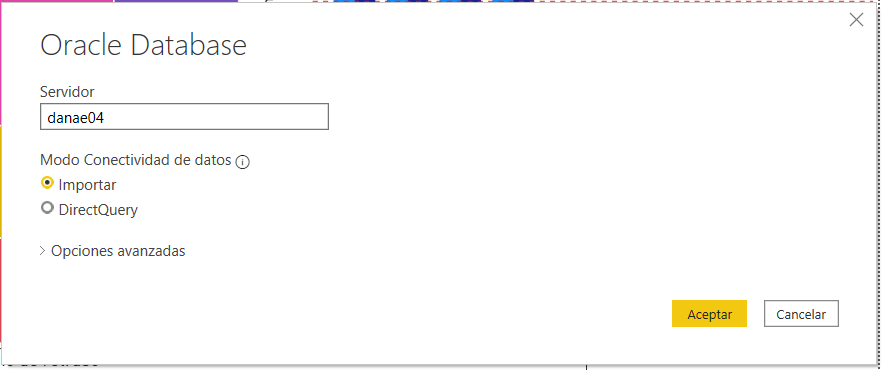
\includegraphics[scale=0.8]{images/cuadroConexion.png}
    \caption{Captura de pantalla del cuadro de conexión de \textit{PowerBI} con \textit{Oracle}}
    \label{fig:cuadroConexion}
\end{figure}

\subsection{Cuadro de credenciales de \textit{PowerBI} al conectar con la base de datos \textit{Oracle}}

\begin{figure}[h!]
    \centering
    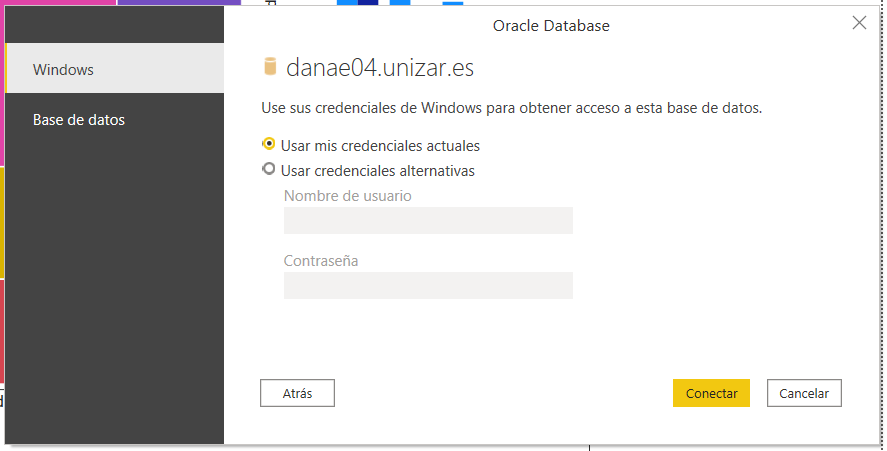
\includegraphics[scale=0.8]{images/cuadroConexionCredenciales.png}
    \caption{Captura de pantalla del cuadro de credenciales de la conexión de \textit{PowerBI} con \textit{Oracle}}
    \label{fig:cuadroConexionCredenciales}
\end{figure}

\newpage
\subsection{Modelo de Datos de \textit{PowerBI}}

\begin{figure}[h!]
    \centering
    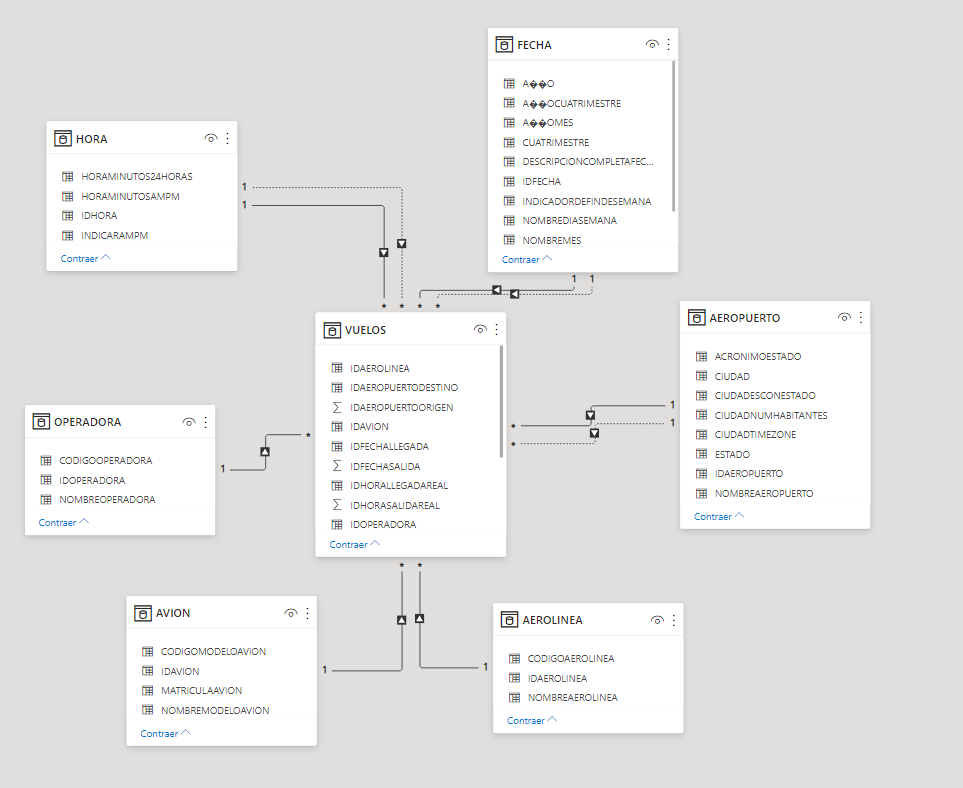
\includegraphics[scale=0.8]{images/modeloDatosPowerBI.png}
    \caption{Captura de pantalla del modelo de datos inferido por \textit{PowerBI}}
    \label{fig:modeloDatos}
\end{figure}

% Anexo de codigos
%\newpage
%\section{Anexo 2: Códigos}


% Bibliografía
\newpage
\addcontentsline{toc}{section}{Referencias}
\bibliographystyle{unsrt}
\bibliography{bibliografia.bib}

\end{document}